% !TEX root = main.tex
% \newpage

\section{Background and Motivation} 
\label{sec:background}

\noindent Virtual memory is ubiquitous in nearly all computing systems
today and is responsible for translating virtual addresses to physical
addresses. Address translation is performed by maintaining an
application {\em page table} in system memory.
Figure~\ref{fig:page_table} shows a typical four-level
hierarchical page table commonly used in computing systems today. Each
node in the page table is 4KB in size and contains 512 8-byte entries
that point to the next node in the page table. The leaf node contains
the physical address mapping. Generally, the page table is sparsely
populated and new nodes are created only when data is referenced. As
such, the typical in-memory storage space for the application page
table is roughly 0.2\% of the total memory footprint (8 bytes of
storage overhead when using 4KB pages).

% Modern processors provide hardware support for address translation
% using the Memory Management Unit (MMU) and Input/Output MMU (IOMMU).
% The MMU handles CPU requests while the IOMMU handles device requests
% (e.g. GPU). 

Figure~\ref{fig:page_table} illustrates a {\em page walk} for a
four-level page table. The Memory Management Unit (MMU) (or page
walker) first consults a predetermined register (e.g. CR3 register on
x86 systems) to determine the physical address for Page Map Level 4
(PML4) or root node of the page table. The MMU indexes PML4 to fetch
the Page Directory Pointer (PDP) or third-level page table (first
memory reference). Next, the MMU indexes the PDP to fetch the Page
Directory (PD) or second-level page table (second memory reference).
Next, the MMU indexes the PD to fetch the first-level of the Page
Table (PT) (third memory reference). Finally, the MMU indexes the PT
(fourth memory reference) to fetch the physical address mapped to the
virtual address.

% \footnote{\noindent \small{In a virtualized environment, a
% page walk by the guest operating system may require up to 16 memory
% references}}.

% \begin{figure}[t] 
% \vspace{0. in}
% \centering
% \centerline{\psfig{file=GRAPHS/motivation_perf_mpki,angle=-90,width=\columnwidth}}
% 
% 	\caption{\small Workloads incur significant performance
% 	overhead due to frequent LLT misses. \normalsize}
% 
% \label{fig:llt_missrate} 
% \vspace{-0.15 in}
% \end{figure}

%\begin{figure}[t] 
%\vspace{0. in}
%\centering
%\centerline{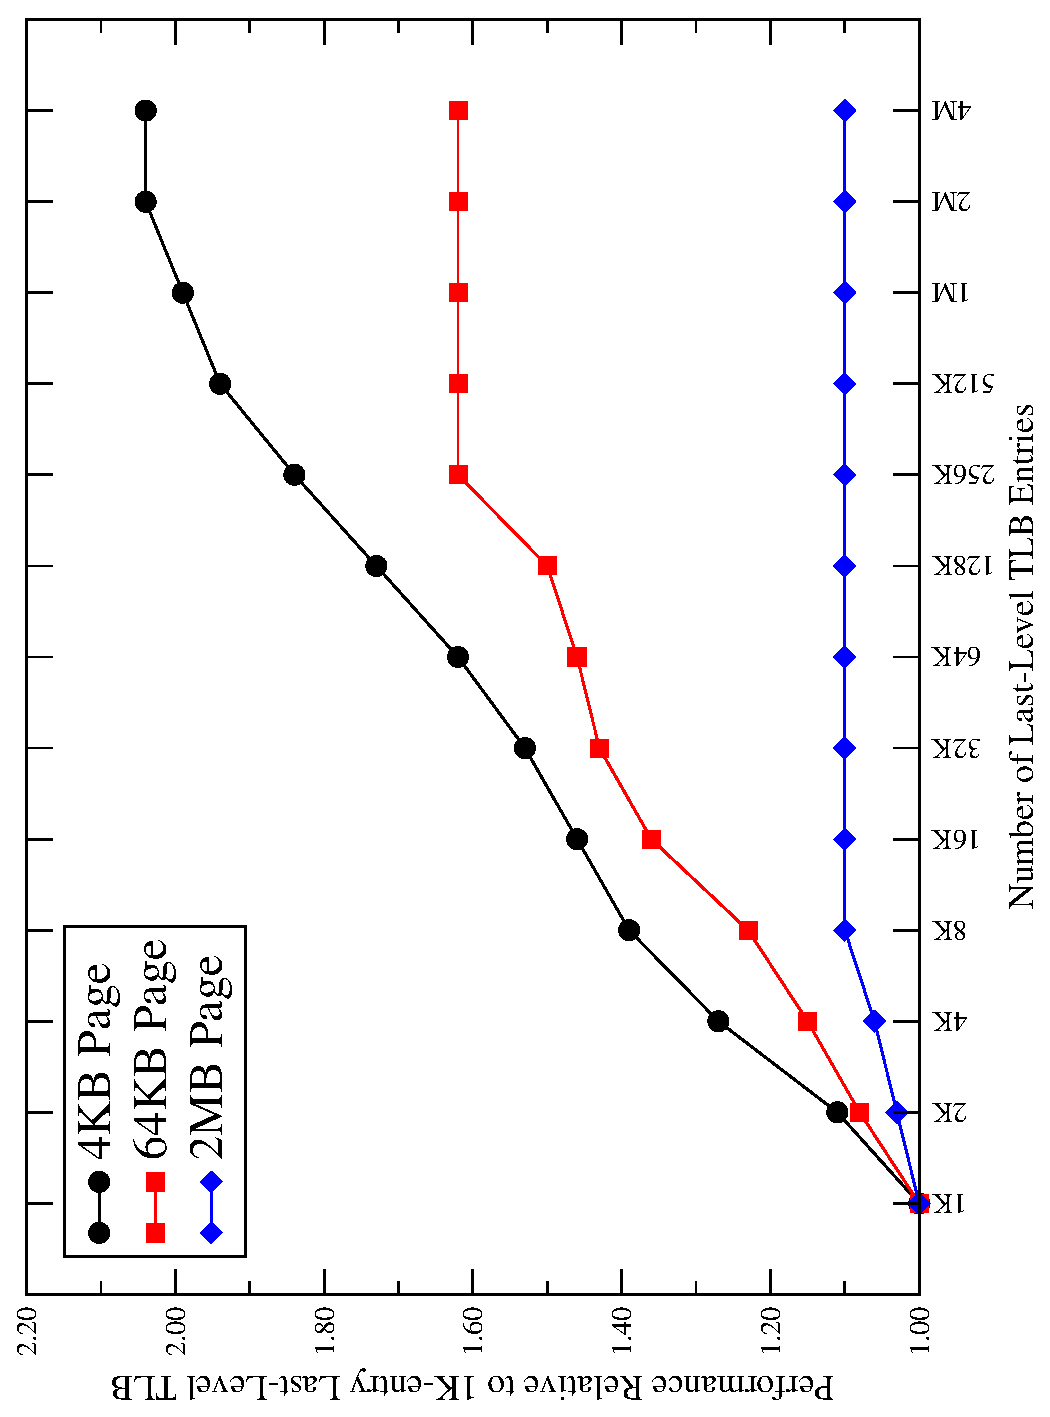
\psfig{file=GRAPHS/tlb_sensitivity,angle=-90,width=\columnwidth}}

%	\caption{\small Performance Sensitivity to LLT Entries. \normalsize}

%\label{fig:tlb_sensitivity} 
%\vspace{-0.15 in}
%\end{figure}

To reduce page table accesses on an LLT miss, commercial processors
employ Page Walk Caches (PWC) for each page table level. PWCs exploit
temporal and spatial locality in the page table access stream and
avoid memory accesses on PWC hits. Consequently, the frequency of TLB
misses and PWC hit rates impacts address translation performance.

\begin {table}[b]
\small
\begin{center} 
\vspace{-0.0 in}
\caption{Workload Behavior with 4KB Page Size}
\vspace{-0. in}
\begin{tabular}{| c | c | c | c | c | }
\hline
  LLT                   & Name     &  LLT-mpki  & \# PT Access    &  Footprint  \\ 
  Sensitivity           &          &    & Per LLT Miss   &             \\ \hline
\multirow{5}{*}{High}   & XSBench  & 90.9       & 1.59         &  3.2 GB  \\
                        & dmr      & 81.3       & 1.81         &  1.5 GB  \\
                        & GUPS     & 92.0       & 2.00         &  15  GB  \\
                        & MaxFlow  & 86.8       & 1.83         &  1.5 GB  \\
                        & MCB      & 69.5       & 1.00         &  100 MB  \\ \hline
\multirow{6}{*}{Medium} & bfs      & 1.45       & 1.06         &  572 MB  \\
                        & LULESH   & 4.64       & 1.49         &  3.7  GB \\
                        & SNAP     & 4.81       & 1.15         &  1.6 GB  \\
                        & UMT      & 3.71       & 1.51         &  1.4 GB  \\
                        & CoMD     & 4.95       & 1.18         &  780 MB  \\
                        & HPGMG    & 6.78       & 1.54         &  4.4 GB  \\ \hline 
\multirow{3}{*}{Low}    & MiniAMR  & 5.58       & 1.62         &  3.3 GB  \\
                        & AMG      & 2.30       & 1.38         &  2.9 GB  \\ 
                        & Nekbone  & 4.36       & 1.29         &  1.1 GB  \\ \hline


\end{tabular}
\label{table:bench_char}
\vspace{-0.2in}
\end{center}
\normalsize
\end{table}


In the previous Section we already motivated increasing TLB
coverage by demonstrating its direct impact on performance in Figure~\ref{fig:tlb_sensitivity}. To provide further insight, Table~\ref{table:bench_char} 
shows the number of LLT misses for the evaluated workloads.
We observe that these workloads incur frequent LLT misses when using 4KB pages. 
To make things worse,
each LLT miss requires more than one memory access to the page table
(maximum of two in some cases). Consequently, these workloads experience
significant performance overheads due to TLB misses. This clearly
motivates the need for reducing the number of memory accesses on an LLT miss in addition to improving LLT coverage. Before
we describe our solutions to address both these problems, we first
provide details on our experimental methodology.

\begin{figure}[t]
\vspace{0. in}
\centering
\centerline{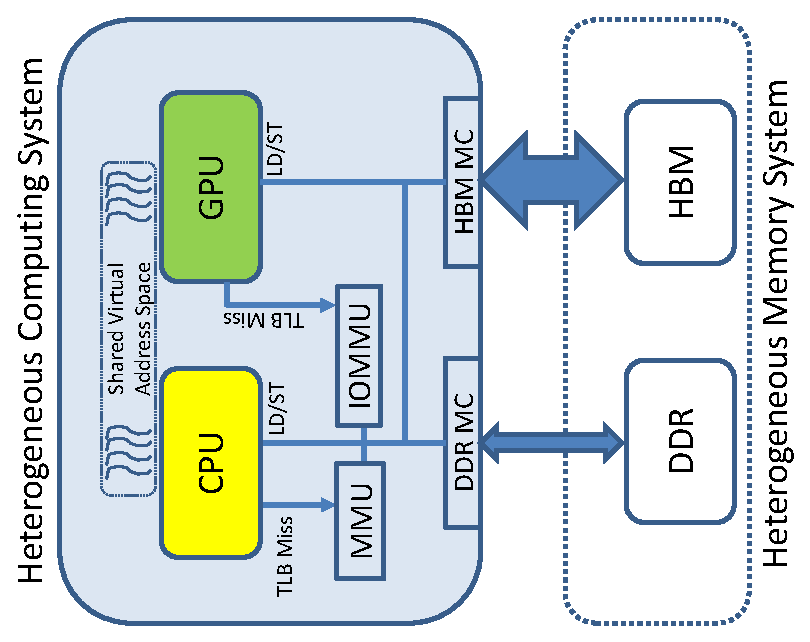
\psfig{file=FIGURES/config,scale=0.4,angle=-90}}

        \caption{\small Baseline System. \normalsize}

\label{fig:config}
\vspace{-0.15 in}
\end{figure}

